\section{V6}
\begin{multicols}{2}
\begin{minipage}{\linewidth}
\subsection{Exceptions and Interrupts}
Der NVIC verarbeitet bis 240 IRQ und einem NMI\\
\begin{tabular}{ll}
    normaler Programmablauf& \rightarrow Background  \\ 
    Exception-Handler& \rightarrow Foreground  \\ 
\end{tabular} 
\end{minipage}

    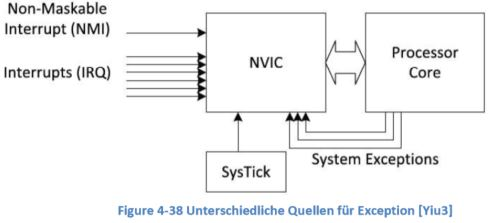
\includegraphics[width=\linewidth]{images/NVICExcp}
\end{multicols}
Exception-Handler für Interrupts werden als INterrupt Service Routine (ISR) bezeichnet.

\subsection{Reset und Reset-Sequenzen}
\subsubsection{Reset}
Es gitb 3 Arten von Reset:\\
\begin{tabular}{ll}
    Power-on Reset& Resettet den gesammten \mu C, auch alle Preripherien und Debug-Komponenten \\ 
    System Reset& Resettet nur den Prozessor nu die Periferien, aber nicht die Debug-Komponenten \\ 
    Processer Reset& Resettet nur den Prozessor\\
\end{tabular}

\subsubsection{Reset Sequenz}
     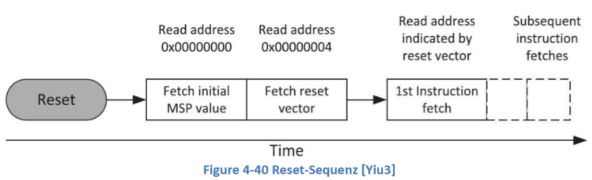
\includegraphics{images/resetsequenz}
\subsection{Spezial-Register}     
Register um Exceptions ein oder auszuschalten:\\
\textbf{\rightarrow PRIMASK,FAULTMASK,BASEPRI}
\begin{multicols}{2}
\subsubsection{PRIMASK}
\begin{itemize}
    \item 1-bit Register
    \item Wenn das aktiv ist, werden NMI-Interrupts erlaubt
    \subitem \rightarrow alle anderen Interrupts werden überdeckt
    \subitem \rightarrow defaultwert= 0, also deaktiviert
\end{itemize}

\subsubsection{FAULTMASK}
\begin{itemize}
    \item 1-bit Register
    \item Wenn das aktiv ist, werden nur noch NMI-INterrups akzeptiert.\newline
    alle anderen Interrupts und Exceptioln-Handlings werden deaktiviert
    \subitem \rightarrow Default-Wert = 0
\end{itemize}
\end{multicols}
\subsubsection{BASEPRI}
\begin{itemize}
    \item Register das bis zu 8 Bits enthalten kann
    \item definiert eine Prioritätsstufe
    \item Hohe Stufe = HOhe Priorität
    \item Wenn das gesetzt wird, werden alle Interrupts mit gleicher oder tieferer Stufe deaktiviert
\end{itemize}

\subsubsection{Control-Register}
Das Kontroll-Register definiert:
\begin{enumerate}
    \item Die Auswahl zwischen MSP (Main-SP) und PSP(Process-SP)
    \item Die Zugriffsstufe un Thread-Mode
    \subitem (Ob Privilegd oder unprivilegd)
    \end{enumerate}
    \begin{multicols}{2}
    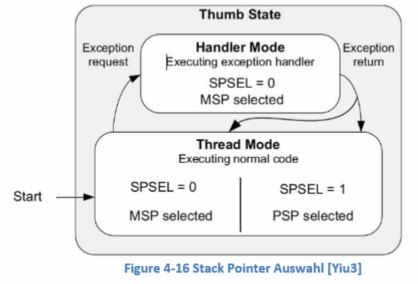
\includegraphics[width=\linewidth]{images/StackPointerAuswahl}
    
         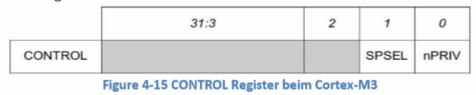
\includegraphics[width=\linewidth]{images/controlRegister}
             \end{multicols}